\documentclass[aspectratio=169]{beamer}
\usetheme{Madrid}
\usecolortheme{seahorse}
\setbeamertemplate{navigation symbols}{}
\setbeamertemplate{footline}[frame number]
\usepackage{booktabs}
\usepackage{graphicx}
\graphicspath{{figs/}}

\title[What a prediction model learns about its questions]{What a prediction model figures out about its test questions}
\subtitle{and the one it learns only roughly}
\author{Wenrui Yuan}
\date{}

\begin{document}

\begin{frame}\titlepage\end{frame}

% ---------------------------------------------------------------------------
\begin{frame}{The setup}
We train a model to do one job, predict whether a learner answers the next
question correctly. Answers can be right or wrong, or graded into a few levels
(right or wrong is two levels, a five point grade is five).
\medskip

To predict well, the model ends up working out three numbers on its own.
\begin{itemize}
\item \textbf{score}, how strong the learner is.
\item \textbf{difficulty}, how hard the question is.
\item \textbf{sharpness}, how clearly a question tells apart strong and weak learners.
\end{itemize}
\medskip

On a sharp question, strong learners almost always get it and weak ones almost
never. On a dull question, everyone is near a coin flip no matter their strength.
\medskip

We never hand the model these numbers. It is graded only on predicting answers.
On made-up data the true numbers are known, so we can check how well the model's
numbers match them, from 0 (no match) to 1 (perfect order).
\end{frame}

% ---------------------------------------------------------------------------
\begin{frame}{The question}
\begin{block}{}
When a model learns only by predicting answers, which of the three numbers does
it get right, how fast, and why?
\end{block}
\medskip

Short answer. It gets the learner's score and the question's difficulty easily.
It struggles with the question's sharpness. The rest of the talk is why, what
helps, and one tempting explanation we tested and ruled out.
\end{frame}

% ---------------------------------------------------------------------------
\begin{frame}{Two of the three numbers are easy, one is not}
\begin{columns}
\begin{column}{0.62\textwidth}

\includegraphics[width=\linewidth]{s1_three_speeds.png}
\end{column}
\begin{column}{0.36\textwidth}
\small
Score and difficulty climb to a near perfect match within the first few to
twenty training steps. Sharpness rises slowly and never quite catches up,
settling a notch below the other two (about 0.93 on the same 0 to 1 scale,
against 0.97 and 0.99).
\medskip

With more answer levels the gap is wider. So the model gets two of the three
numbers almost for free and works much harder for the third.
\end{column}
\end{columns}
\end{frame}

% ---------------------------------------------------------------------------
\begin{frame}{Why sharpness is the hard one}
\begin{columns}
\begin{column}{0.6\textwidth}
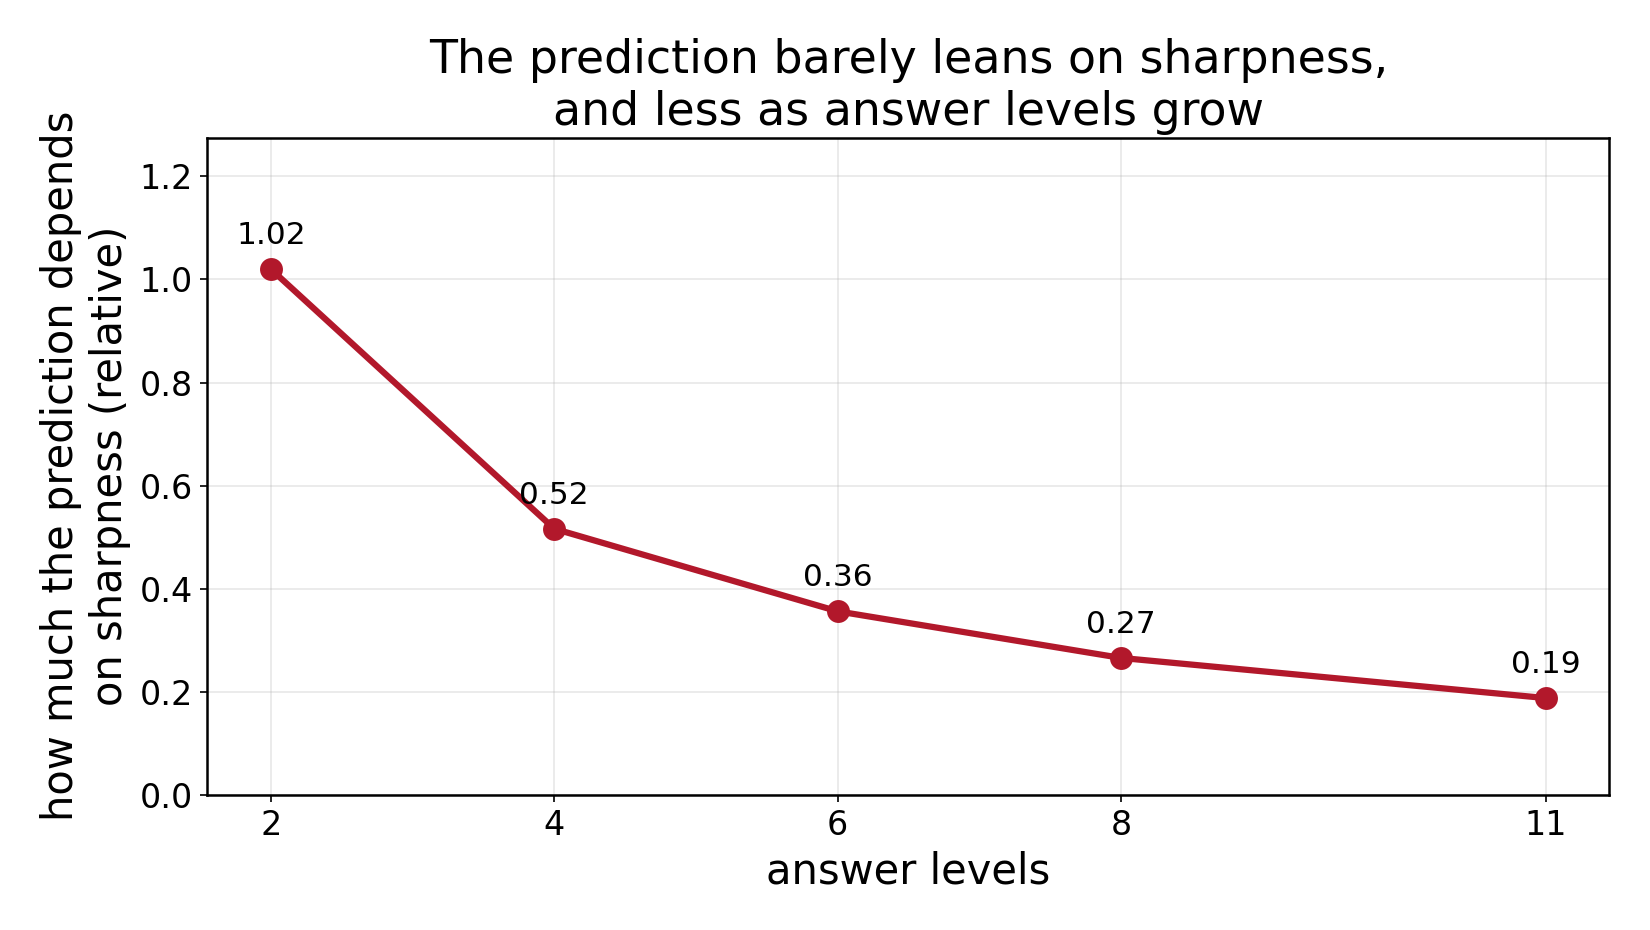
\includegraphics[width=\linewidth]{s4_why_hard.png}
\end{column}
\begin{column}{0.38\textwidth}
\small
A model can only learn a number as well as its prediction leans on that number.
\medskip

The prediction leans heavily on score and difficulty. It barely leans on
sharpness. Sharpness only changes the prediction for learners whose strength is
close to a question's difficulty. For everyone far above or far below, the answer
is nearly settled either way, so sharpness makes almost no difference. Add more
answer levels and the prediction leans on it even less.
\medskip

That weak signal is the main reason sharpness is slow and unreliable.
\end{column}
\end{columns}
\end{frame}

% ---------------------------------------------------------------------------
\begin{frame}{A fix aimed straight at the hard number}
\begin{columns}
\begin{column}{0.58\textwidth}
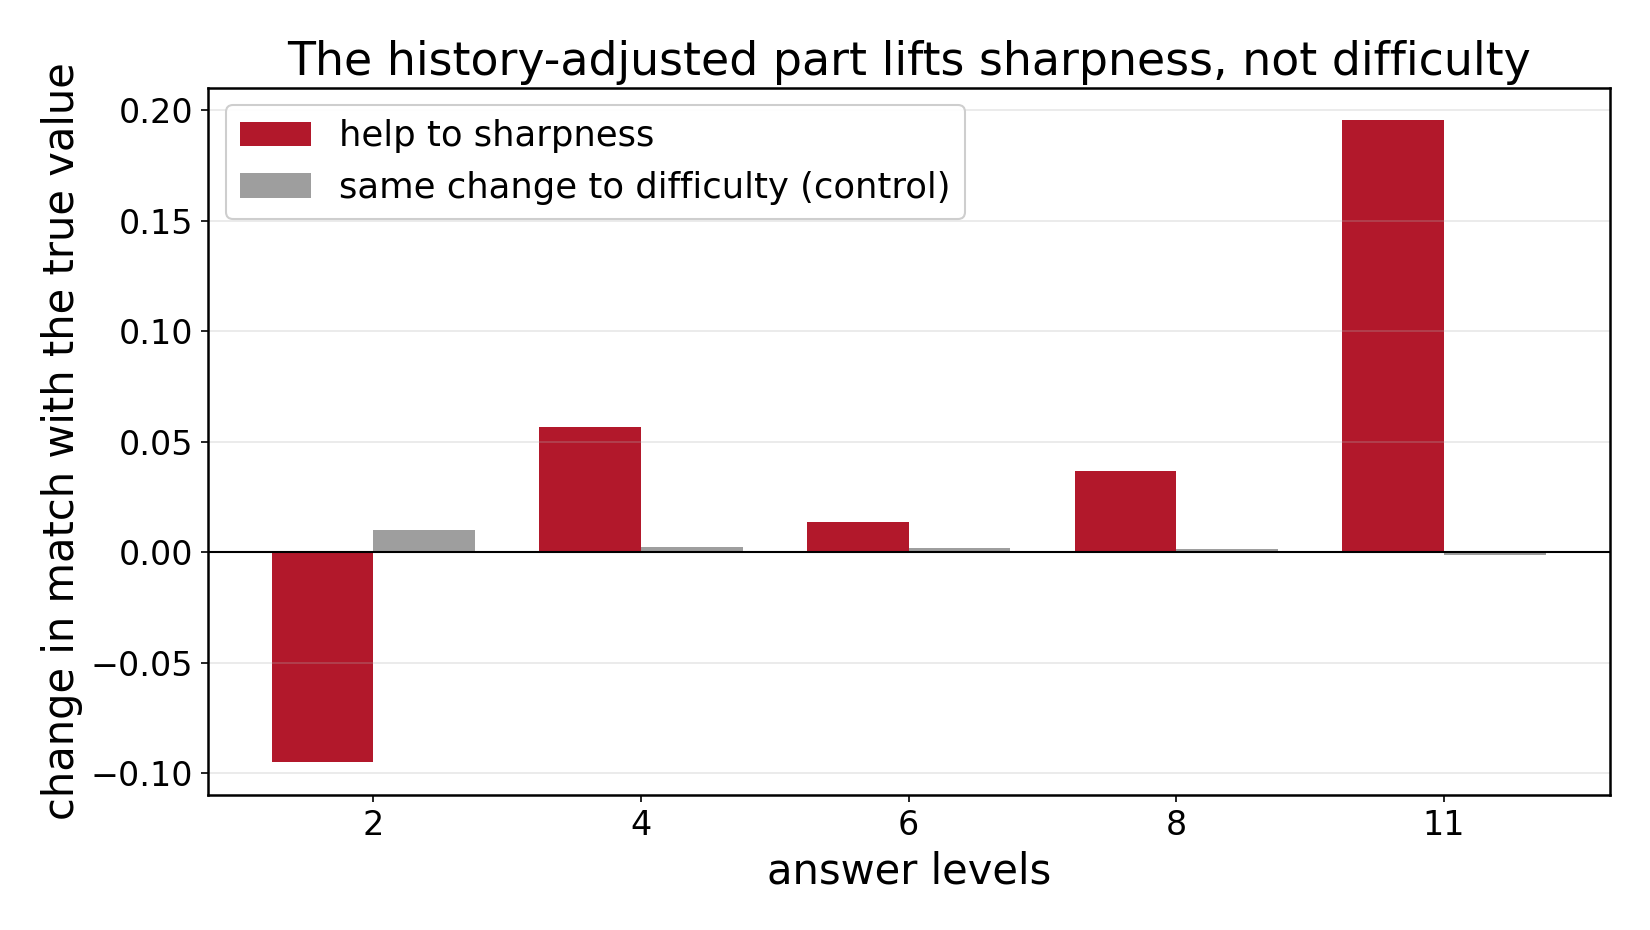
\includegraphics[width=\linewidth]{s2_sharpness_help.png}
\end{column}
\begin{column}{0.4\textwidth}
\footnotesize
Give each question's sharpness two parts, a fixed part for the question plus a
small extra part that shifts with the learner's recent answers.
\medskip

The match to true sharpness improves, mostly by getting there faster and more
reliably, and the gain grows with more answer levels, up to about $+0.20$ at
eleven.
\medskip

Two controls make it real. The same change to difficulty does almost nothing
(grey bars), and a size-matched plain model does not close the gap.
\medskip

Caveat, at two answer levels it slightly hurts, so this helps richer grading
scales, not the simplest right or wrong case.
\end{column}
\end{columns}
\end{frame}

% ---------------------------------------------------------------------------
\begin{frame}{A tempting explanation we tested and ruled out}
\begin{columns}
\begin{column}{0.58\textwidth}
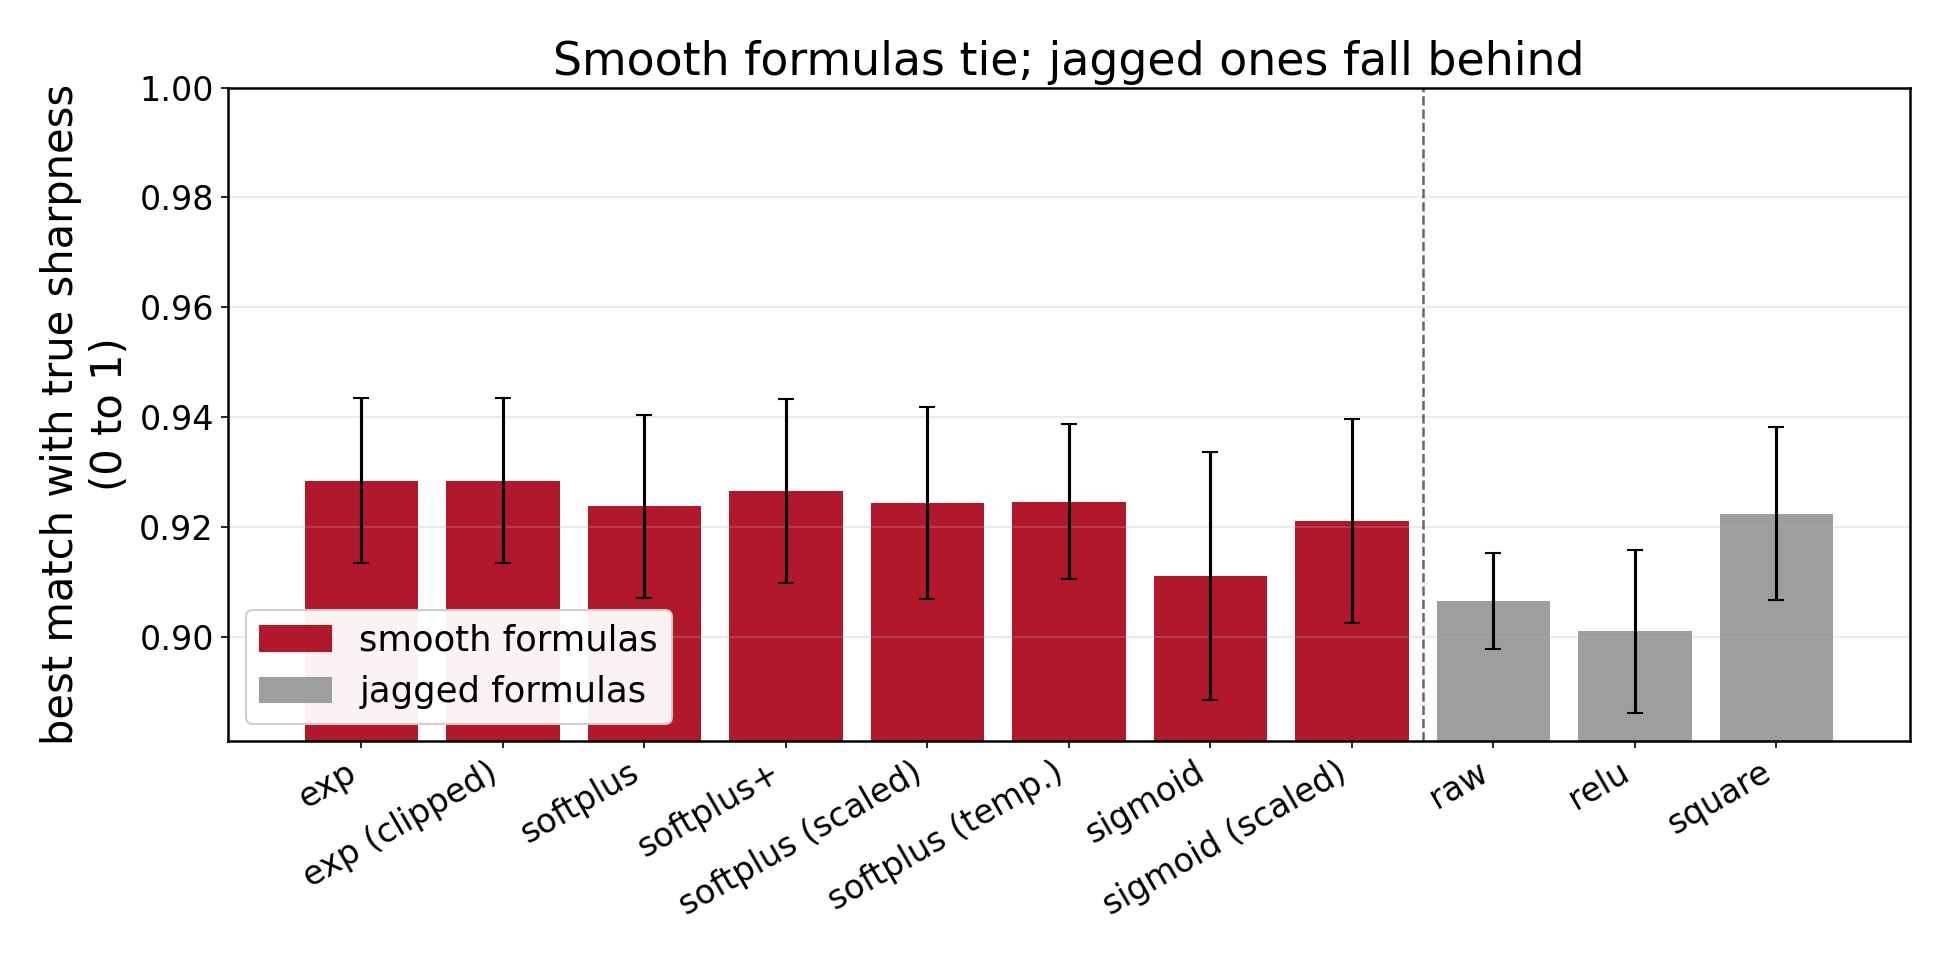
\includegraphics[width=\linewidth]{s3_formula_distractor.png}
\end{column}
\begin{column}{0.4\textwidth}
\footnotesize
Sharpness must be a positive number. A common trick is to learn a free number
and pass it through an always-positive formula. We suspected one formula, the
exponential, was the secret.
\medskip

Compared fairly, each given the same starting point and its own best settings,
they all tie. Only the crude options lag, the one that can still slip negative
and the one that flattens to zero and stops responding.
\medskip

A follow-up idea, that the exponential helps by changing the training step
sizes, also failed its own test. Being positive and smooth helps, the
exponential does not. What actually helps is the previous slide's fix, giving
sharpness its own dedicated part of the model.
\end{column}
\end{columns}
\end{frame}

% ---------------------------------------------------------------------------
\begin{frame}{How far to trust the history part}
We planted a real, known link between a question's sharpness and the learner's
strength, then asked the history-adjusted part to find it.
\medskip

\begin{itemize}
\item It picks up the \textbf{direction} of the link.
\item It badly \textbf{underestimates the size} of the link.
\item It shows a little signal even when we planted none, so a small adjustment can be noise, not a real link.
\end{itemize}
\medskip

So we read the history part for direction, not for amount. A bigger history
adjustment is not the same as a stronger real effect.
\end{frame}

% ---------------------------------------------------------------------------
\begin{frame}{Takeaway}
\begin{block}{One line}
A model trained only to predict answers learns each question number only as well
as the prediction leans on it.
\end{block}
\medskip
\begin{itemize}
\item Sharpness is the number the prediction barely leans on, so it is learned
slowly and only roughly.
\item Giving sharpness a fixed part plus a history-adjusted part helps, more so
with more answer levels. It is a gain in speed and reliability, and it recovers
the order of sharpness, not its exact size.
\item We ruled out the idea that a special positive formula was the key.
Positivity and smoothness matter, the formula does not.
\end{itemize}
\medskip
\footnotesize Honest limits, made-up data, a few repeats, one model type. Next
step, a check on real learner data.
\end{frame}

\end{document}
